\section{Современные подходы оптимизации с ограничениями.}

\subsection{Современные подходы}
\begin{enumerate}
    \item \textbf{Self-Adaptive Fitness Formulation}
    \begin{itemize}
        \item Делает предпочтение особям, не удовлетворяющим ограничениям, которые недалеки от границы, и у которых хорошие значения целевых критериев
        \item Штрафные коэффициенты рассчитываются, исходя из минимальных и максимальных значений выхода за пределы границы
        \item Farmani R., Wright J.A. Self-Adaptive Fitness Formulation for Constrained Optimization // IEEE
        Transactions on Evolutionary Computation. — 2003. — Vol. 7, no. 5. — P. 445–455
    \end{itemize}


    \item \textbf{Adaptive Segregation Constraint Handling EA}
    \begin{itemize}
        \item Семейство алгоритмов, разработанных S. Hamida и M. Schoenauer в 2000–2002 годах
        \item Поддерживать штрафные коэффициенты таким образом, чтобы доля особей $T$, удовлетворяющих ограничениям, была около $T_0$:
        \begin{itemize}
            \item  $T < T_0$: умножить коэффициенты на $Y$
            \item  $T > T_0$: разделить коэффициенты на $Y$
        \end{itemize}
        \item Коэффициенты инициализируются, исходя из того, как начальная популяция удовлетворяет ограничениям
        \item Если $T < T0$, запускать скрещивание особей по разные стороны границы
        \item  \textbf{«Segregation Selection»}: $K < T_0$ особей, удовлетворяющих ограничениям, обязательно проходит в следующее поколение, остальные особи отбираются по оштрафованной приспособленности

    \end{itemize}

    \item \textbf{Стохастическое ранжирование}
    \begin{itemize}
        \item «Сломанная» сортировка пузырьком. Обычно $0.4 \leq T \leq 0.5$
        \item Работает хорошо, до сих пор является одним из лучших алгоритмов
    \end{itemize}
    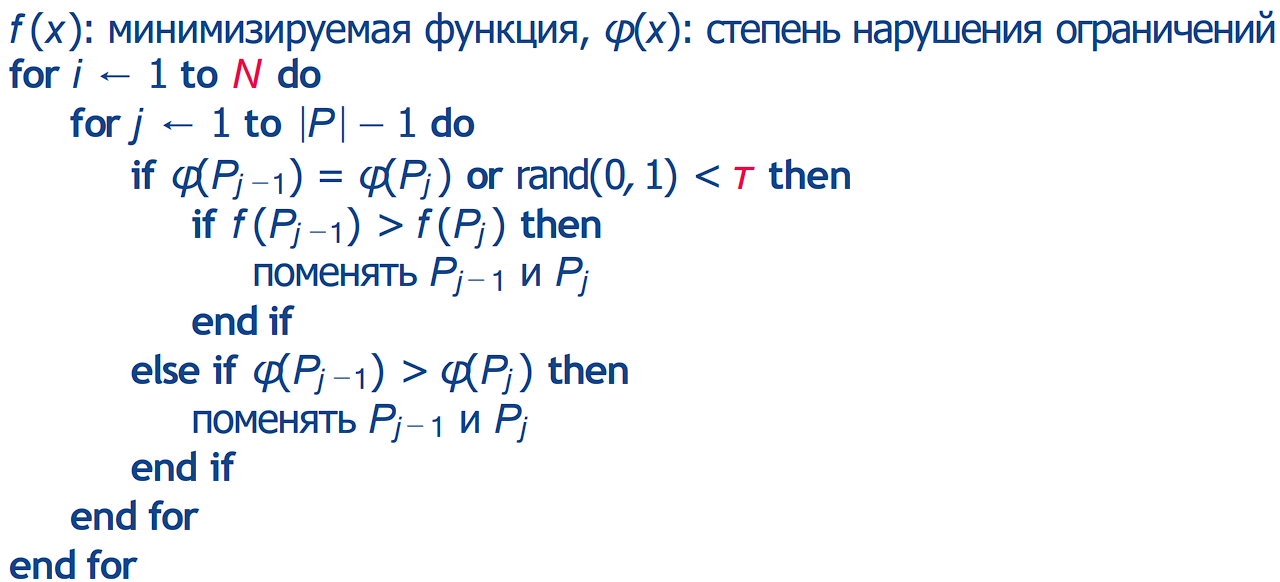
\includegraphics[scale=0.5]{images/formula_min_func.png}

\end{enumerate}

\subsection{Специальные представления и операторы}
\begin{itemize}
    \item \textbf{Homomorphous Mapping}
    \begin{itemize}
        \item [~] Если известна форма подпространства поиска, удовлетворяющего ограничениям, постараться генерировать особи из этого подпространства с помощью преобразующей функции из $R^n$, сохраняющей топологические свойства
        \item [+] если получилось, можно забыть об ограничениях
        \item [+] относительно просто для выпуклых подпространств
        \item [--] требует знания вида ограничений
        \item [--] если подпространство невыпукло, сложно и вычислительно затратно

    \end{itemize}
\end{itemize}

\subsection{Методы починки особей}
\begin{enumerate}
    \item \textbf{Скорее «техники»}
    \begin{itemize}
        \item Требуют и знаний о виде ограничений и способа трансформации особи с целью удовлетворения ограничений
        \item Крайне сильно зависит от задачи
    \end{itemize}

    \item \textbf{Дарвин и Ламарк}
    \begin{itemize}
        \item Нужно ли чинить не только фенотип, но и генотип?
        \item Иногда говорят «никогда», иногда говорят «всегда», в некоторых работах эмпирически установлена оптимальность починки 15 процентов генотипов для большого числа разных задач
        \item Исправить генотип не всегда возможно
    \end{itemize}

\end{enumerate}

\subsection{Разделение ограничений и целевых функций}
\begin{enumerate}
    \item \textbf{Коэволюция}
    \begin{itemize}
        \item Одна популяция удовлетворяет ограничениям и минимизирует целевую функцию, другая не удовлетворяет и минимизирует нарушение ограничений
        \item Популяции как-то взаимодействуют путем «переселения» особей
    \end{itemize}

    \item \textbf{Многокритериальная оптимизация}
    \begin{itemize}
        \item Интерпретирует каждое ограничение как еще один минимизируемый критерий
        \item Нужны изменения: другие подходы к разнообразию в популяции, некоторые критерии равнее других, и т.д.
    \end{itemize}

    \item \textbf{Лексикографическое сравнение}
    \begin{itemize}
        \item  Минимизировать нарушение ограничений по одному, затем оптимизировать критерии: просто, иногда эффективно
    \end{itemize}
\end{enumerate}
